\documentclass{article}

\usepackage{fancyhdr}
\usepackage{extramarks}
\usepackage{amsmath}
\usepackage{amsthm}
\usepackage{amssymb}
\usepackage{amsfonts}
\usepackage{tikz}
\usepackage[plain]{algorithm}
\usepackage{algpseudocode}

%
% Basic Document Settings
%

\topmargin=-0.45in
\evensidemargin=0in
\oddsidemargin=0in
\textwidth=6.5in
\textheight=9.0in
\headsep=0.25in

\linespread{1.2}

\pagestyle{fancy}
\rhead{\hmwkAuthorName}
\lhead{\hmwkClass: \hmwkTitle}


\renewcommand\headrulewidth{0.4pt}
\renewcommand\footrulewidth{0.4pt}
\renewcommand{\proofname}{\textit{\textbf{ Proof.}}}

% \setlength\parindent{0pt}

%
% Create Problem Sections
%

\newcommand{\enterProblemHeader}[1]{
    \nobreak\extramarks{}{Problem \arabic{#1} continued on next page\ldots}\nobreak{}
    \nobreak\extramarks{Problem \arabic{#1} (continued)}{Problem \arabic{#1} continued on next page\ldots}\nobreak{}
}

\newcommand{\exitProblemHeader}[1]{
    \nobreak\extramarks{Problem \arabic{#1} (continued)}{Problem \arabic{#1} continued on next page\ldots}\nobreak{}
    \stepcounter{#1}
    \nobreak\extramarks{Problem \arabic{#1}}{}\nobreak{}
}

\setcounter{secnumdepth}{0}
\newcounter{partCounter}
\newcounter{homeworkProblemCounter}
\setcounter{homeworkProblemCounter}{1}
\nobreak\extramarks{Problem \arabic{homeworkProblemCounter}}{}\nobreak{}

%
% Homework Problem Environment
%
% This environment takes an optional argument. When given, it will adjust the
% problem counter. This is useful for when the problems given for your
% assignment aren't sequential. See the last 3 problems of this template for an
% example.
%
\newenvironment{homeworkProblem}[1][-1]{
    \ifnum#1>0
        \setcounter{homeworkProblemCounter}{#1}
    \fi
    \section{Problem \arabic{homeworkProblemCounter}}
    \setcounter{partCounter}{1}
    \enterProblemHeader{homeworkProblemCounter}
}{
    \exitProblemHeader{homeworkProblemCounter}
}


\newcommand{\hmwkTitle}{Assignment 5}
\newcommand{\hmwkClass}{Manifold Learning and Sparse Representation}
\newcommand{\hmwkAuthorName}{\textbf{ZHANG Yuan}, 1601111332 }
\date{}
%
% Title Page
%

\title{
    \textmd{\textbf{\hmwkClass:\ \hmwkTitle}}\\
}

\author{\hmwkAuthorName}

\renewcommand{\part}[1]{\textbf{\large Part \Alph{partCounter}}\stepcounter{partCounter}\\}

%
% Various Helper Commands
%

% Useful for algorithms
\newcommand{\alg}[1]{\textsc{\bfseries \footnotesize #1}}

% For derivatives
\newcommand{\deriv}[1]{\frac{\mathrm{d}}{\mathrm{d}x} (#1)}

% For partial derivatives
\newcommand{\pderiv}[2]{\frac{\partial}{\partial #1} (#2)}

% Integral dx
\newcommand{\dx}{\mathrm{d}x}

% Alias for the Solution section header
\newcommand{\solution}{\textbf{\large Solution}}

% Probability commands: Expectation, Variance, Covariance, Bias
\newcommand{\E}{\mathrm{E}}
\newcommand{\Var}{\mathrm{Var}}
\newcommand{\Cov}{\mathrm{Cov}}
\newcommand{\Bias}{\mathrm{Bias}}

\begin{document}

\maketitle
\section{Exercise 76.}
\begin{proof}
Becasue Frobenius norm is unitary invariant, we have
\begin{align*}
    L = \Vert \mathbf{X} - \mathbf{A} \Vert_F^2 = &\Vert \mathbf{U^{T}XU} - \mathbf{\Lambda} \Vert_F^2 \\
    = &\Vert \mathbf{\tilde X} - \mathbf{\Lambda} \Vert_F^2 \\
    = &\sum_{i}(\tilde{x}_{ii}-\lambda_i)^2 + 2\sum_{i<j}x_{ij}^2\\
    \geq & \sum_{i}(\tilde{x}_{ii}-\lambda_i)^2,
\end{align*}
where $\mathbf{A = U\Lambda U^T}$ is the eigen-decomposition of $\mathbf A$ and $\tilde{\mathbf X}\textbf{} \triangleq \mathbf{U^{T}XU}$. 

Since $dim\{\mathbf{a} | \mathbf{a^TXa}>0\} = rank(\mathbf X) \leq r$, the number of non-zero diagonal elements (i.e. $\{x_ii\}$) of $\mathbf X$ is less or equal than $r$. Besides, the fact that $X$ is p.s.d. implies all the non-zero diagonal elements should be positive. Thus, the solution to $\min. L$ is $\mathbf{\tilde X} = diag(\max(\lambda_1,0),\max(\lambda_r,0),0,..,0)$ so that $\mathbf{X = U_r\max(\Lambda_r,0)U_r^T}$.
\end{proof}


\section{Exercise 77.}
The visualization of CMDS with $k =2$ is shown as in Fig. 1. \textit{Square Euclidean distance} that is widely used in many clustering scenarios is used in my settings.
\begin{figure}[htbp]
    \centering
    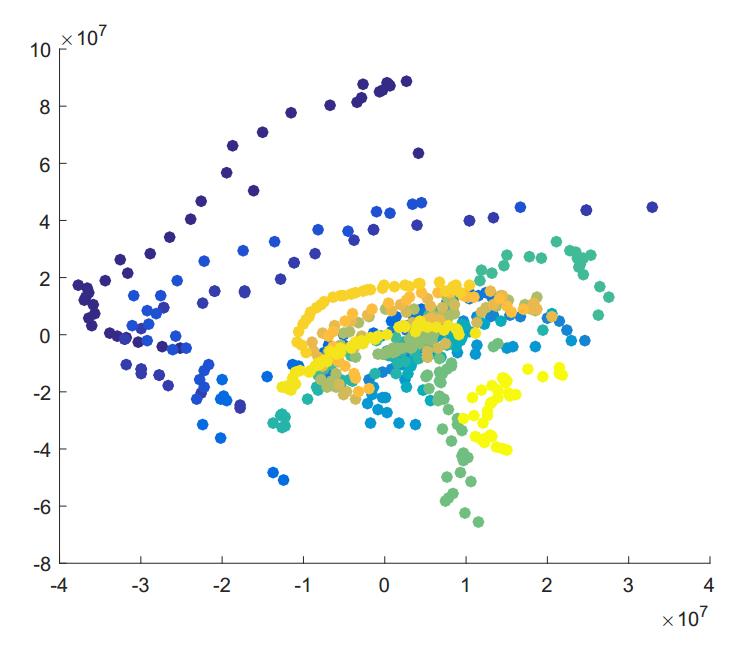
\includegraphics[scale = 0.25]{fig1}
    \caption{2-D embedding visualization w/ square Euclidean distance.}
\end{figure}

\section{Exercise 93.}
The first 12 faces of each person are used for training and another 5 faces for testing. The average recognition rate is $0.8103$. 
\end{document}